%%%%%%%%%%%%%%%%%%%%%%%%%%%%%%%%%%%%

\section{3.3. Distribuição geométrica}

%%%%%%%%%%%%%%%%%%%%%%%%%%%%%%%%%%%%

\subsection{Distribuição Bernoulli}

\begin{frame}
\frametitle{Experimento de Milgram}

\twocol{0.6}{0.4}{

\begin{itemize}
\justifying
\item Stanley Milgram, psicólogo da Universidade de Yale, conduziu uma série de experimentos sobre obediência à autoridade a partir de 1963.
\justifying
\item O pesquisador (E) ordena que o professor (T), que é o sujeito do experimento, aplique choques elétricos a um aluno (L) toda vez que este responder a uma pergunta incorretamente.

\end{itemize}

}
{
\begin{center}
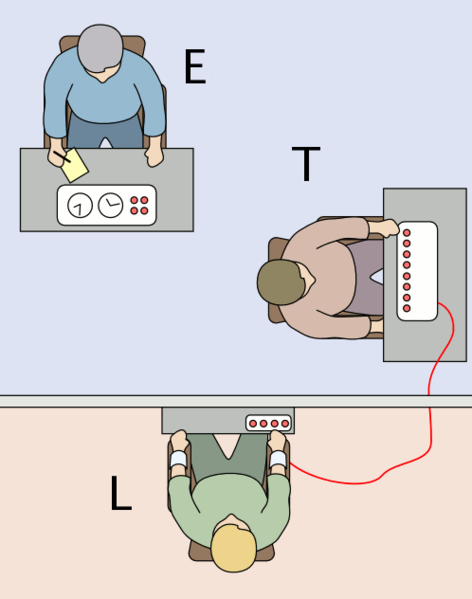
\includegraphics[width=\textwidth]{3-3_geometric_distribution/milgram.png}
\end{center}
\justifying
\ct{\webURL{http://en.wikipedia.org/wiki/File:Milgram_Experiment_v2.png}}
}

\end{frame}


%%%%%%%%%%%%%%%%%%%%%%%%%%%%%%%%%%%%

\begin{frame}
\frametitle{Experimento de Milgram (cont.)}

\begin{itemize}
\justifying
\item O aluno é na verdade um ator, e os choques elétricos não são reais, mas um som pré-gravado é tocado toda vez que o professor administra um choque elétrico.
\justifying
\item Esse experimento mediu a vontade dos participantes do estudo em obedecer a uma figura de autoridade que os instruiu a realizar atos que conflitassem com sua consciência pessoal.
\justifying
\item Milgram descobriu que cerca de 65\% das pessoas obedeceriam à autoridade e dariam tais choques.
\justifying
\item Ao longo dos anos, outras pesquisas sugeriram que esse número é aproximadamente consistente entre as comunidades e o tempo.

\end{itemize}

\end{frame}


%%%%%%%%%%%%%%%%%%%%%%%%%%%%%%%%%%%%

\begin{frame}
\frametitle{Variáveis aleatórias de Bernoulli}

\begin{itemize}
\justifying
\item Na experiência de Milgram cada pessoa pode ser tratada como uma \hl{tentativa}.
\justifying
\item A pessoa é considerada como \hl{sucesso} se ela se recusar a administrar um choque e como \hl{falha} se ela administrar o choque.
\justifying
\item Como apenas 35\% das pessoas se recusaram a administrar o choque, a \hl{probabilidade de sucesso} é \mathhl{p = 0.35}.
\justifying
\item Quando uma particular tentativa tem apenas dois resultados possíveis, ela é chamada de \hl{variável aleatória de Bernoulli}.

\end{itemize}

\end{frame}

%%%%%%%%%%%%%%%%%%%%%%%%%%%%%%%%%%%%

\subsection{Distribuição geométrica}

\begin{frame}
\frametitle{Distribuição geométrica}

{\small
\justifying
\dq{A Dra. Smith quer repetir os experimentos de Milgram, mas ela só quer testar pessoas até encontrar alguém que não esteja disposto a aplicar choques. Qual é a probabilidade de ela parar o experimento depois da primeira pessoa?}

\[ P(1^{0}~pessoa~recusa) = 0.35 \]

\pause
\justifying
\dq{... a terceira pessoa?}
\[ P(1^{0}~e~2^{0}~choque,~3^{0}~recusa) = \slot{S}{0.65} \times \slot{S}{0.65} \times  \slot{R}{0.35} = 0.65^2 \times 0.35 \approx 0.15 \]
}
\pause
\end{frame}

%%%%%%%%%%%%%%%%%%%%%%%%%%%%%%%%%%%%

\begin{frame}
\frametitle{Distribuição geométrica}
{\small
\dq{... a décima pessoa?}
\soln{
\pause
\[ P(9~choque,~10^{0}~recusa) = \underbrace{\slot{S}{0.65} \times \cdots \times \slot{S}{0.65}}_{9~deste} \times  \slot{R}{0.35} = 0.65^9 \times 0.35 \approx 0.0072 \]
}
}

\end{frame}

%%%%%%%%%%%%%%%%%%%%%%%%%%%%%%%%%%%%

\begin{frame}
\frametitle{Distribuição geométrica (cont.)}
\justifying
A \hl{Distribuição geométrica} descreve o tempo de espera até um sucesso para variáveis aleatórias Bernoulli \hl{independentes e identicamente distribuídas (iid)}.
\pause
\begin{itemize}
\justifying
\item independência: os resultados dos ensaios não afetam uns aos outros.
\justifying
\item idêntico: a probabilidade de sucesso é a mesma para cada tentativa.
\end{itemize}
\pause
\formula{Probabilidades geométricas}{Se $ p $ representa a probabilidade de sucesso, então $ (1-p) $ representa a probabilidade de falha e $ n $ representa número de tentativas independentes \[P(sucesso~na~n^{esima}~tentativa) = (1-p)^{n-1} p\]}

\end{frame}
%%%%%%%%%%%%%%%%%%%%%%%%%%%%%%%%%%%%


\begin{frame}
\frametitle{Exemplo}
\justifying
\pq{Podemos calcular a probabilidade de obter um 6 pela primeira vez na sexta jogada de um dado utilizando a distribuição geométrica? Note que o sucesso (sair um 6) e o fracasso (não sair um 6) estão claramente definidos e um ou outro deve acontecer para cada tentativa.}

\begin{enumerate}[(a)]
\justifying
\item não, no lançamento de um dado há mais de dois resultados possíveis
\justifying
\only<1>{\item sim, pois}
\justifying
\soln{\only<2>{\item \orange{sim, pois}}}
\end{enumerate}

\soln{
\only<2>{
\[P(6~na~6^{a}~jogada) = \pr{ \frac{5}{6} }^5 \pr{ \frac{1}{6} } \approx 0.067 \]
}
}

\end{frame}

%%%%%%%%%%%%%%%%%%%%%%%%%%%%%%%%%%%%

\begin{frame}
\frametitle{Valor esperado}
\justifying
\dq{Quantas pessoas a Dra. Smith espera testar antes de encontrar a primeira que se recusará a administrar o choque?}

\pause
\justifying
O valor esperado, ou a média, de uma distribuição geométrica é definida como $\frac{1}{p}$.
\[ \mu = \frac{1}{p} = \frac{1}{0.35} = 2.86 \]

\pause
\justifying
Ela deve testar 2,86 pessoas antes de encontrar o primeiro que se recusa a administrar o choque.

\pause
\justifying
Mas como ela pode testar um número não-inteiro de pessoas?

\end{frame}

%%%%%%%%%%%%%%%%%%%%%%%%%%%%%%%%%%%%

\begin{frame}
\frametitle{Valor esperado e sua variabilidade}
\justifying
\formula{Média e desvio padrão da distribuição geométrica}{
\[ \mu = \frac{1}{p} \qquad \qquad \sigma = \sqrt{\frac{1-p}{p^2}} \] 
}

\pause

\begin{itemize}
\justifying
\item Voltando à experiência da Dra. Smith:

\[ \sigma = \sqrt{\frac{1-p}{p^2}} = \sqrt{\frac{1-0.35}{0.35^2}} = 2.3 \]

\pause
\justifying
\item Espera-se que a Dra. Smith teste 2,86 pessoas antes de encontrar o primeiro que se recusa a administrar o choque, mais ou menos 2,3 pessoas.

\pause
\justifying
\item Esses valores só fazem sentido no contexto de repetir o experimento muitas vezes.

\end{itemize}

\end{frame}

%%%%%%%%%%%%%%%%%%%%%%%%%%%%%%%%%%%%

